\documentclass[9pt]{beamer}

\usepackage[T1]{fontenc}
\usepackage[utf8]{inputenc}
\usepackage[frenchb]{babel}
\usepackage{eurosym}

\usepackage{multirow}

\usepackage{graphicx}


\newcommand\host{{\it host} }
\newcommand\device{{\it device} }


% --------- BEGIN STYLE BEAMER ---------
\usetheme{Madrid}
\definecolor{ECNBleu}{HTML}{102648}
\definecolor{ECNJaune}{HTML}{FAB600}

\setbeamercolor{frametitle}{bg=ECNBleu,fg=white} %le titre de la frame, en haut
\setbeamercolor{title in head/foot}{bg=ECNJaune,fg=ECNBleu} %barre bas, milieu
\setbeamercolor{author in head/foot}{bg=ECNBleu,fg=ECNJaune} %barre bas, gauche
\setbeamercolor{date in head/foot}{bg=ECNBleu,fg=ECNJaune} %barre bas, droit
\setbeamercolor{section in head/foot}{bg=ECNJaune,fg=ECNBleu} %haut gauche
\setbeamercolor{subsection in head/foot}{bg=ECNBleu,fg=ECNBleu} %haut droite
\setbeamercolor{title}{bg=ECNBleu,fg=white}
\setbeamercolor{block title}{fg=white,bg=ECNBleu}

%\setbeamercolor{normal text}{bg=IUTBleuFonce} %texte
\setbeamercolor{item}{bg=ECNBleu}
\setbeamercolor{subitem}{bg=ECNJaune}
\setbeamercolor{description item}{fg=couleurEmph}
\setbeamercolor{section in toc}{fg=ECNBleu}
%\setbeamercolor{subsubitem}{bg=IUTBleuFonce}

%structure (eq emph dans beamer)
\setbeamercolor{emph}{fg=couleurEmph}
% ----------------------------

\usepackage{listings}

\lstdefinestyle{customc}{
  belowcaptionskip=1\baselineskip,
  breaklines=true,
  frame=L,
  xleftmargin=\parindent,
  language=C,
  showstringspaces=false,
  basicstyle=\tiny\ttfamily,
  keywordstyle=\bfseries\color{green!40!black},
  commentstyle=\itshape\color{purple!40!black},
  identifierstyle=\color{blue},
  stringstyle=\color{orange},
}

\lstset{escapechar=@,style=customc}

\newenvironment<>{questionblock}[1]{%
\setbeamercolor{block title}{bg=ECNJaune,fg=ECNBleu}%
\begin{block}#2{#1}}{\end{block}}

\title[GPGPU]{Programmation sur Processeur Graphique}

\subtitle[\ldots]{
---\\Partie 9 : Algorithme parallèle de réduction}
\author[P.-E. Hladik]{Pierre-Emmanuel Hladik\\\tiny pierre-emmanuel.hladik@ec-nantes.fr}
\institute[Centrale Nantes]{}
\date{\today}

\begin{document}
 \frame{\titlepage}


%%%%%%%%%%%%%%%%%%%%%%%%%%
\begin{frame}[plain]
\frametitle{Qu'est-ce q'un algorithme de réduction ?}
      \centering
      \begin{block}{}
	Agglomérer un ensemble de valeurs d'entrée en une seule valeur en utilisant une "opération de réduction", exemples :
      	\begin{itemize}
		\item Max
		\item Min
		\item Somme
		\item  Produit
	\end{itemize}

	\end{block}  
\end{frame}
%%%%%%%%%%%%%%%%%%%%%%%%%%
\begin{frame}[plain]
\frametitle{Algorithme séquentiel en O(N)}
      \centering
      \begin{block}{}
      \begin{enumerate}
	\item 	Initialiser le résultat en tant que valeur d'identité pour l'opération de réduction :
	\begin{itemize}
		\item La plus petite valeur possible pour le Max
		\item Valeur la plus élevée possible pour le  Min
		\item 0 pour la Somme
		\item 1 pour le Produit
	\end{itemize}
	\item Itérer sur les valeurs d'entrée l'opération de réduction entre la valeur du résultat et la valeur actuelle
\end{enumerate}

	\end{block}  
	      \begin{block}{}
		\begin{itemize}
		\item N opérations de réduction effectuées pour N valeurs d'entrée
		\item Chaque valeur d'entrée n'est visitée qu'une seule fois -- algorithme en O(N)
		\item Il s'agit d'un algorithme efficace sur le plan du calcul
	\end{itemize}
		\end{block}  
\end{frame}
%%%%%%%%%%%%%%%%%%%%%%%%%%%
\begin{frame}[plain]
\frametitle{Stratégie de partionnement et d'aglomération}
      \centering
      \begin{block}{}
      	Une stratégie couramment utilisée pour le traitement de grands ensembles de données d'entrée
      	\begin{itemize}
		\item pas d'ordre requis des éléments de traitement dans un ensemble de données
		\item Diviser l'ensemble de données en plus petits morceaux
		\item Avoir un thread pour traiter un morceau
		\item Construire un arbre de réduction pour aglomérer les résultats de chaque morceau
	\end{itemize}
	\end{block}  
\end{frame}
%%%%%%%%%%%%%%%%%%%%%%%%%%
\begin{frame}[plain]
\frametitle{Algo parallèle d'arbre de réduction en log(N) étapes}
\begin{center}
	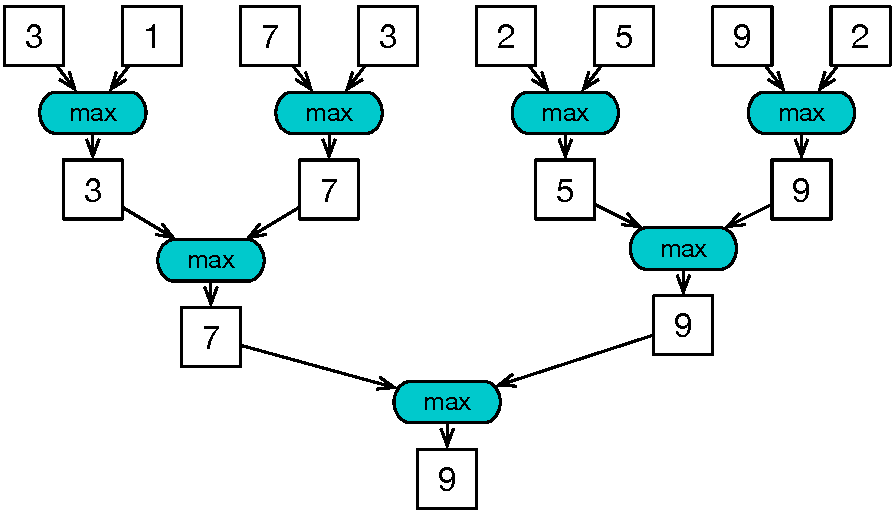
\includegraphics[scale=0.6]{./figures-pdf/red_tree_max}
\end{center}
\end{frame}
%%%%%%%%%%%%%%%%%%%%%%%%%%
\begin{frame}[plain]
\frametitle{Analyse rapide}
\begin{block}{}
	Pour $n$ valeurs l'arbre de réduction effectue:
      	\begin{itemize}
		\item (1/2)$n$ + (1/4)$n$ + (1/8)$n$ + ...  = (1-(1/$n$))$n$ = $n$-1 opérations en log ($n$) étapes
	      	\begin{itemize}
			\item Exemple : le traitement de 1 000 000 de valeurs prend 20 étapes (en supposant que nous disposions de ressources d'exécution suffisantes)
		\end{itemize}
		\medskip
		\item Parallélisme moyen ($n$-1)/log($n$)\\
	      	\begin{itemize}
			\item Pour N = 1 000 000, le parallélisme moyen est de 50 000
			\item Toutefois, le pic de ressources nécessaires est de 500 000
		\end{itemize}
		\medskip
		\item C'est un algorithme parallèle performant en terme de travail
	      	\begin{itemize}
			\item La quantité de travail effectuée est comparable à celle d'un algorithme séquentiel efficace	
%			\item Remarque : de nombreux algorithmes parallèles ne fonctionnent pas efficacement
		\end{itemize}

	\end{itemize}
\end{block}  
\end{frame}
%%%%%%%%%%%%%%%%%%%%%%%%%%
\begin{frame}[plain]
\frametitle{Exemple : réduction d'un maximum}
\begin{block}{Implémentation parallèle}
      	\begin{itemize}
		\item Chaque thread compare 2 valeurs à chaque étape
		\item Réduit par 2 le nombre de thread à chaque étape
		\item Utilise $\log(n)$ étapes pour $n$ éléments et $n/2$ threads
	\end{itemize}
\end{block}  

\begin{block}{Exemple d'utilisation de la mémoire partagée sur une somme}
	\begin{itemize}
%		\item Le vecteur initial est dans la mémoire globale du device
%		\item La mémoire partagée contient une somme partielle
		\item Au départ, la mémoire partagée contient le vecteur initial
		\item Chaque étape rapproche la somme partielle de la somme
		\item La somme finale sera dans l'élément 0 du vecteur partagée
		\item Réduit le trafic global de mémoire grâce à la lecture et à l'écriture de valeurs
		\item La taille maximale des blocs doit être inférieure ou égale à 2048
	\end{itemize}
\end{block}  
\end{frame}
%%%%%%%%%%%%%%%%%%%%%%%%%%
\begin{frame}[plain]
\frametitle{Exemple : réduction d'une somme (schéma)}
\begin{center}
	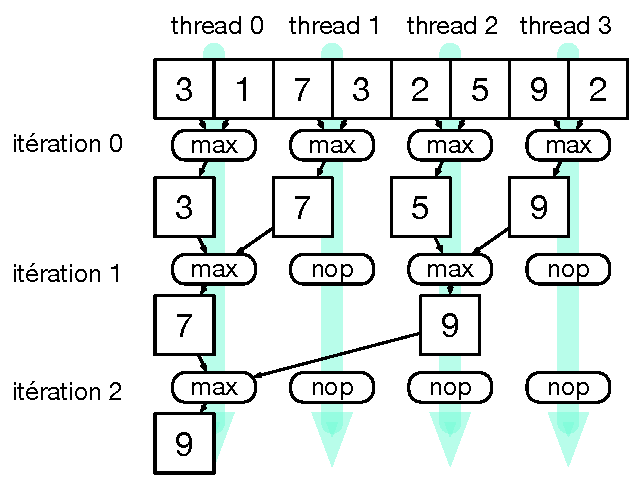
\includegraphics[scale=0.6]{./figures-pdf/red_thread}
\end{center}
\end{frame}
%%%%%%%%%%%%%%%%%%%%%%%%%%
\begin{frame}[plain, fragile]
\frametitle{Exemple : implémentation naïve}

	\begin{itemize}
		\item Chaque block dispose de {\tt 2*BlockDim.x} éléments
		\item Chaque thread charge 2 éléments dans la mémoire partagée
	\end{itemize}

\begin{lstlisting}[language=C]

__global__
void redux(float* input, float* ouput) {

  __shared__ float max[2*BLOCK_SIZE];

  int tx = threadIdx.x;
  int start = 2 * blockIdx.x * blockDim.x;
  
  // write data in shared memory
  max[tx] = input[start + tx];
  max[blockDim + tx] = input[start + blockDim.x + tx];

  for (int stride = 1; stride <= blockDim.x;  stride *= 2) 
  {
    __syncthreads();
    if (tx % stride == 0)
	max[2 * tx] = ( (max[2 * tx] > max[2 * tx + stride]) ? max[2 * tx] : max[2 * tx + stride]);
  }
  
  ouput[blockIdx.x] = max[0];
  
}
 \end{lstlisting}
\end{frame}

%%%%%%%%%%%%%%%%%%%%%%%%%%
\begin{frame}[plain, fragile]
\frametitle{Commentaires sur l'implémentation naïve (divergence)}

	A chaque itération, deux chemins de flux de contrôle ({\bf divergence}) seront parcourus séquentiellement pour chaque $warp$ :
	\begin{itemize}
		\item Les threads qui effectuent des comparaison et les threads qui n'en effectuent pas
		\item Les threads qui n'effectuent pas de comparaison "bloquent" des ressources d'exécution\bigskip
	\end{itemize}
	La moitié ou moins des threads seront en cours d'exécution après la première étape
	\begin{itemize}
		\item Tous les threads d'indices impairs sont inactifs après la première étape
		\item Après la 5e étape, des warps entier dans chaque bloc échouent le test conditionnel (une mauvaise utilisation des ressources mais aucune divergence)
		\item Cela peut durer un certain temps, jusqu'à 6 étapes supplémentaires (stride = 32, 64, 128, 256, 512, 1024), où chaque warp active n'a qu'un thread "productif". 
	\end{itemize}


\end{frame}

%%%%%%%%%%%%%%%%%%%%%%%%%%
\begin{frame}[plain]
\frametitle{Toujours regrouper les threads "productifs"}
\begin{center}
	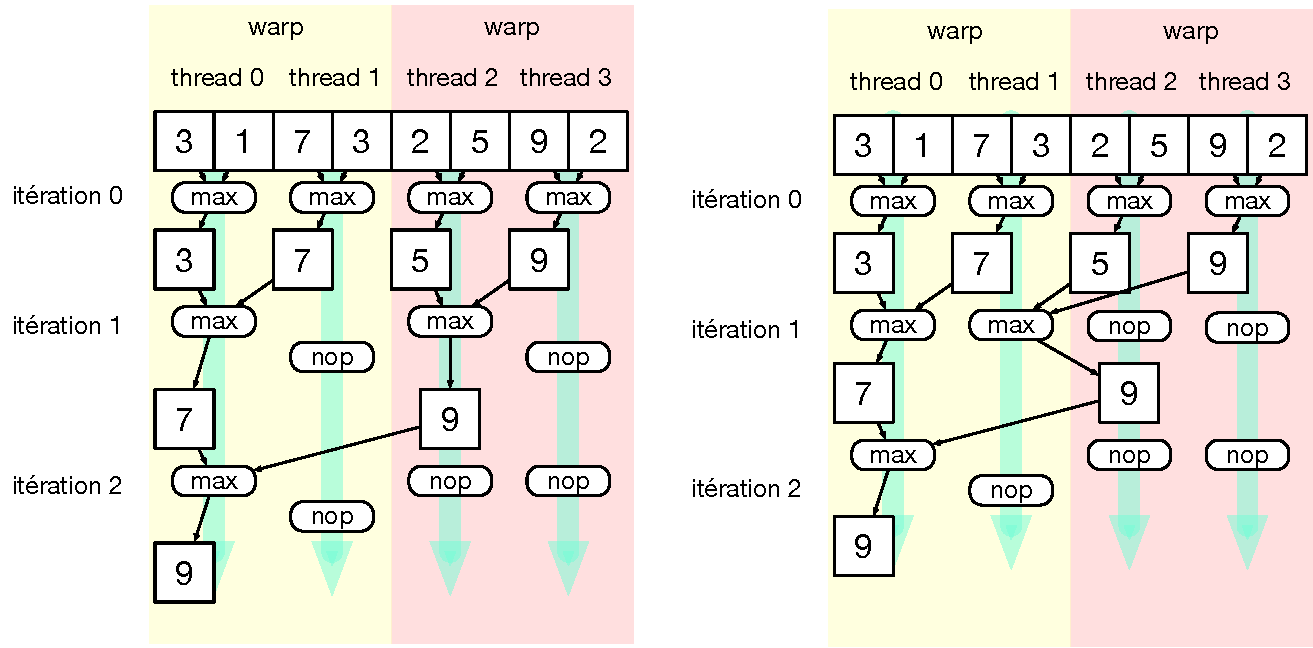
\includegraphics[scale=0.5]{./figures-pdf/red_warp}
\end{center}
\end{frame}
%%%%%%%%%%%%%%%%%%%%%%%%%%
\begin{frame}[plain, fragile]
\frametitle{Exemple : implémentation plus efficace}


\begin{lstlisting}[language=C]

__global__
void redux(float* input, float* ouput) {

  __shared__ float max[2*BLOCK_SIZE];

  int tx = threadIdx.x;
  int start = 2 * blockIdx.x * blockDim.x;
  
  max[t] = input[start + tx];
  max[blockDim + tx] = input[start + blockDim.x + tx];

  for (int stride = blockDim.x; stride > 0; stride /= 2)
  {
    __syncthreads();
    if (tx < stride)
	max[2 * tx] = ( (max[2 * tx] > max[2 * tx + stride]) ? max[2 * tx] : max[2 * tx + stride]);
  }
  ouput[blockIdx.x] = max[0];
}
 \end{lstlisting}

%\begin{lstlisting}[language=C]
%
%__global__
%void redux(float* input, float* ouput) {
%  __shared__ float partialSum[2*BLOCK_SIZE];
%
%  int t = threadIdx.x;
%  int start = 2*blockIdx.x*blockDim.x;
%  
%  partialSum[t] = input[start + t];
%  partialSum[blockDim+t] = input[start + blockDim.x+t];
%
%  for (int stride = blockDim.x; stride > 0; stride /= 2)
%  {
%    __syncthreads();
%    if (t < stride)
%      partialSum[2*t] += partialSum[2*t+stride];
%  }
%  ouput[blockIdx.x] = partialSum[0];
%}
% \end{lstlisting}
\end{frame}

%%%%%%%%%%%%%%%%%%%%%%%%%%
\begin{frame}[plain]
\frametitle{Un peu de pratique avec le TD 9}

\begin{block}{Objectifs}
\begin{itemize}
	\item Observer l’influence des warps
	\item Mettre en œuvre un algorithme d’arbre de réduction
\end{itemize}
\end{block}
\end{frame}
%%%%%%%%%%%%%%%%%%%%%%%%%%

\end{document}